\documentclass[11pt]{article}

\usepackage{amsmath, amssymb, bbold, mathabx, dsfont, multicol, enumitem}
\usepackage{tikz, pgf, pgfplots, pgfkeys}
\usetikzlibrary{calc,matrix,arrows}
\usepackage{amsthm, thmtools}
\usepackage{fancyhdr}
\usepackage{graphicx}
\usepackage[headings]{fullpage}
\usepackage{rotating, hyperref}
\usepackage{graphicx, caption, subcaption, empheq}
 \usepackage{indentfirst}
 
\def \N { \mathds{N} }
\def \Z { \mathds{Z} }
\def \Q { \mathds{Q} }
\def \R { \mathds{R} }
\def \C { \mathds{C} }
\def \H { \mathbb{H}}
\def \F { \mathbb{F} }
\def \T { \mathds{T} }
\def \RP { \mathds{R}P }
\def \pt { \{ \text{pt} \} }
\def \Ker { \text{Ker} }
\def \Im { \text{Im} }

\newcommand{\pd}[2] {\frac{\partial #1}{\partial #2}}
\newcommand{\chpt}[1] { \section*{#1 } \markright{ #1} }

\setlength{\parskip}{2ex plus 0.5ex minus 0.2ex}

\begin{document}
\pagestyle{fancy}
\rhead{Chris LeBailly}
\lhead{Homework 6: Null Models} %CHECK ASSIGNMENT NUMBER!

\section{Project Overview} 

In this project we are attempting to find how likely it is than an ORF of length 388 could occur by chance.  The simplest way to model this is to compute the GC frequency for the species in question, then find the probability of a start codon followed by 387 non-stop codons.  A slightly more sophisticated way is to count 3-mers and use those counts to compute the probability of a start codon followed by 387 non-stop codons.  These are the first two null models we examine.

The main focus of this project was to do a more sophisticated simulation.  The third null model we look at assumes the ORF is on the revers strand of a gene in S.solfataricus.  We first generate a random ORF of length 560.  We do this by taking a start codon, then adding 559 non-stop codons, picked according the codon preference table.  We then take the reverse compliment of this and search for the longest ORF.  The length is recorded.  This is repeated several times (100,000 times in our work) and the distribution of lengths is studied.  We use this to see how likely it is to find an ORF of length 388.  The final null model is similar, but instead of randomly generating ORFs of length 560, we randomly generate a series of codons that codes for THSA\_SULSH, using the codon biases of S.solfataricus.

\section{Results}

\subsection{Null Model 1}

In this null model we use the genome for S.solfataricus to compute the GC-content.  We use an 0-order Markov model to compute the odds of different codons.  Based on 1-mer counts, we find that the probability of G+C is 0.35787.  The probability of seeing an ORF of length 388 is 
\[P(\text{ORF of length 388}) = P(\text{Start Codon}) \cdot (1-P(\text{Stop Codon}))^{387} \]
where $P(\text{Start Codon}) = P(\text{A})P(\text{T})P(\text{G}) = 0.018445$ and $P(\text{Stop Codon}) = P(\text{T})P(\text{A})P(\text{A}) + P(\text{T})P(\text{A})P(\text{G}) + P(\text{T})P(\text{G})P(\text{A}) = 0.069986$. The double-stranded genome contains 5984490 bases.  We find that
\[\text{E-value} = 5984490 \cdot P(\text{ORF of length 388}) = 7.0519 \times 10^{-08}\]
which means we can reject this null model.

\subsection{Null Model 2}
In this null model we count 3-mers in the genome for S.solfataricus.  In this model, the probability of seeing an ORF of length 388 is
\[P(\text{ORF of length 388}) = P(\text{Start Codon}) \cdot (1-P(\text{Stop Codon}))^{387} \]
where $P(\text{Start Codon}) = P(\text{ATG}) = 0.01567$ and $P(\text{Stop Codon}) = P(\text{TAA}) + P(\text{TAG}) + P(\text{TGA}) = 0.070484$.  Since there are 5984486 3-mers in this genome, we find that
\[\text{E-value} = 5984486 \cdot P(\text{ORF of length 388}) = 4.8708 \times 10^{-08}\]
which means we can reject this null model.

\subsection{Null Model 3} 
In this null model we randomly generate ORFs of length 560.  After the start codon we randomly pick 559 nonstop codons, where the likelihood of picking a nonstop codon is given by the codon preference table for S.solfataricus.  After this ORF is generated, we take the reverse compliment and find the longest ORF.  We repeat this 100,000 times to get a distribution of ORF lengths.  Figure \ref{fig:Model3Gum} shows our data fitted to a Gumbel distribution.  Figure \ref{fig:Model3Log} shows our data fitted to a lognormal distribution.

\begin{figure}[!htb]
        \centering
        \begin{subfigure}[b]{0.49\textwidth}
                \centering
		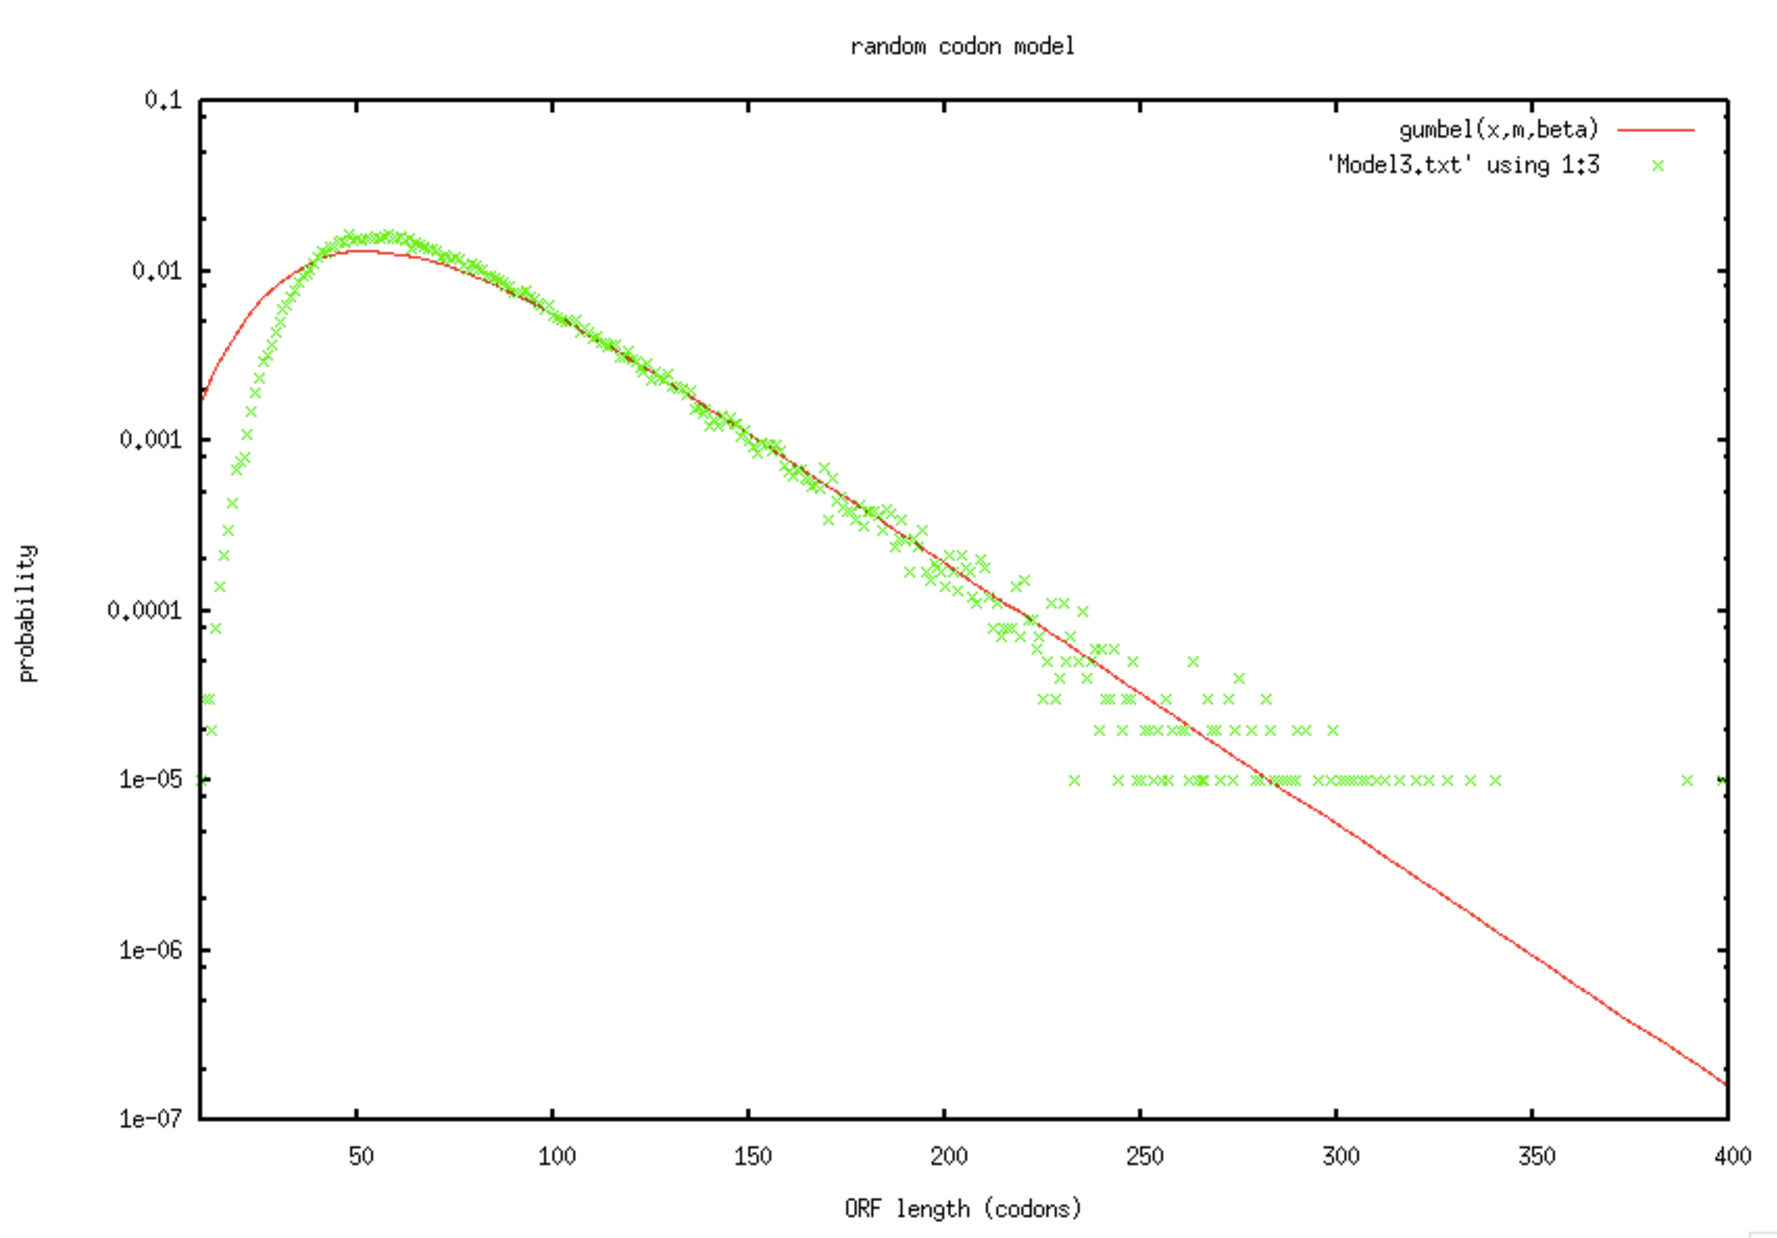
\includegraphics[width=\textwidth]{Model3GumProb.pdf} 
		\caption{Probability vs. ORF length}
        \end{subfigure}
        \begin{subfigure}[b]{0.49\textwidth}
                \centering
		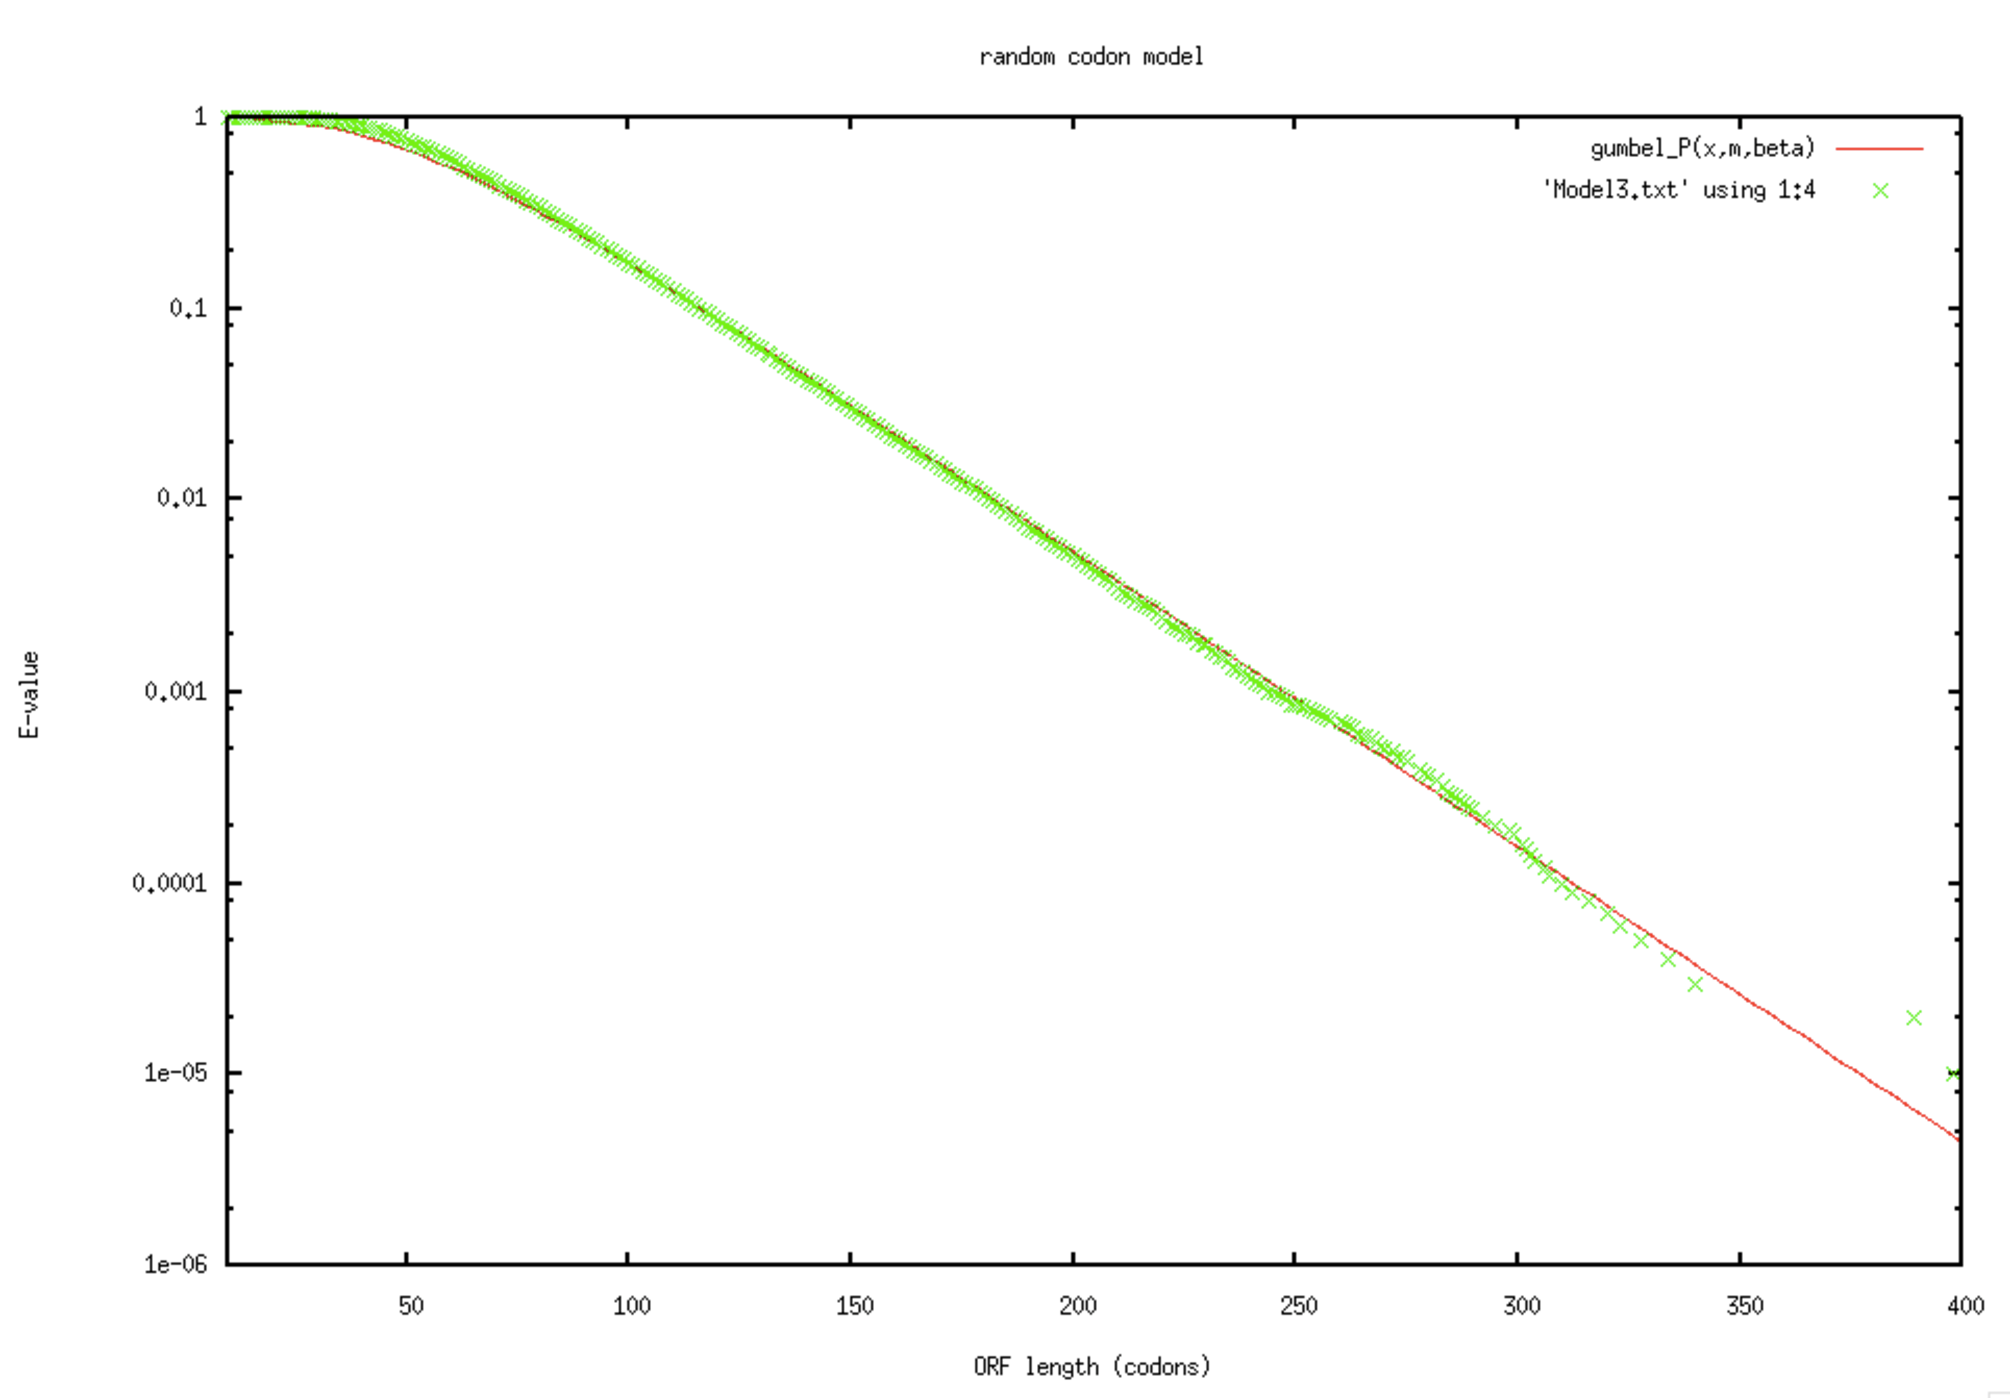
\includegraphics[width=\textwidth]{Model3GumE.pdf} 
		\caption{E-Value vs. ORF length}
        \end{subfigure}

        \caption{Gumbel Distribution for Random Codon Model}\label{fig:Model3Gum}
\end{figure}

\begin{figure}[!htb]
        \centering
        \begin{subfigure}[b]{0.49\textwidth}
                \centering
		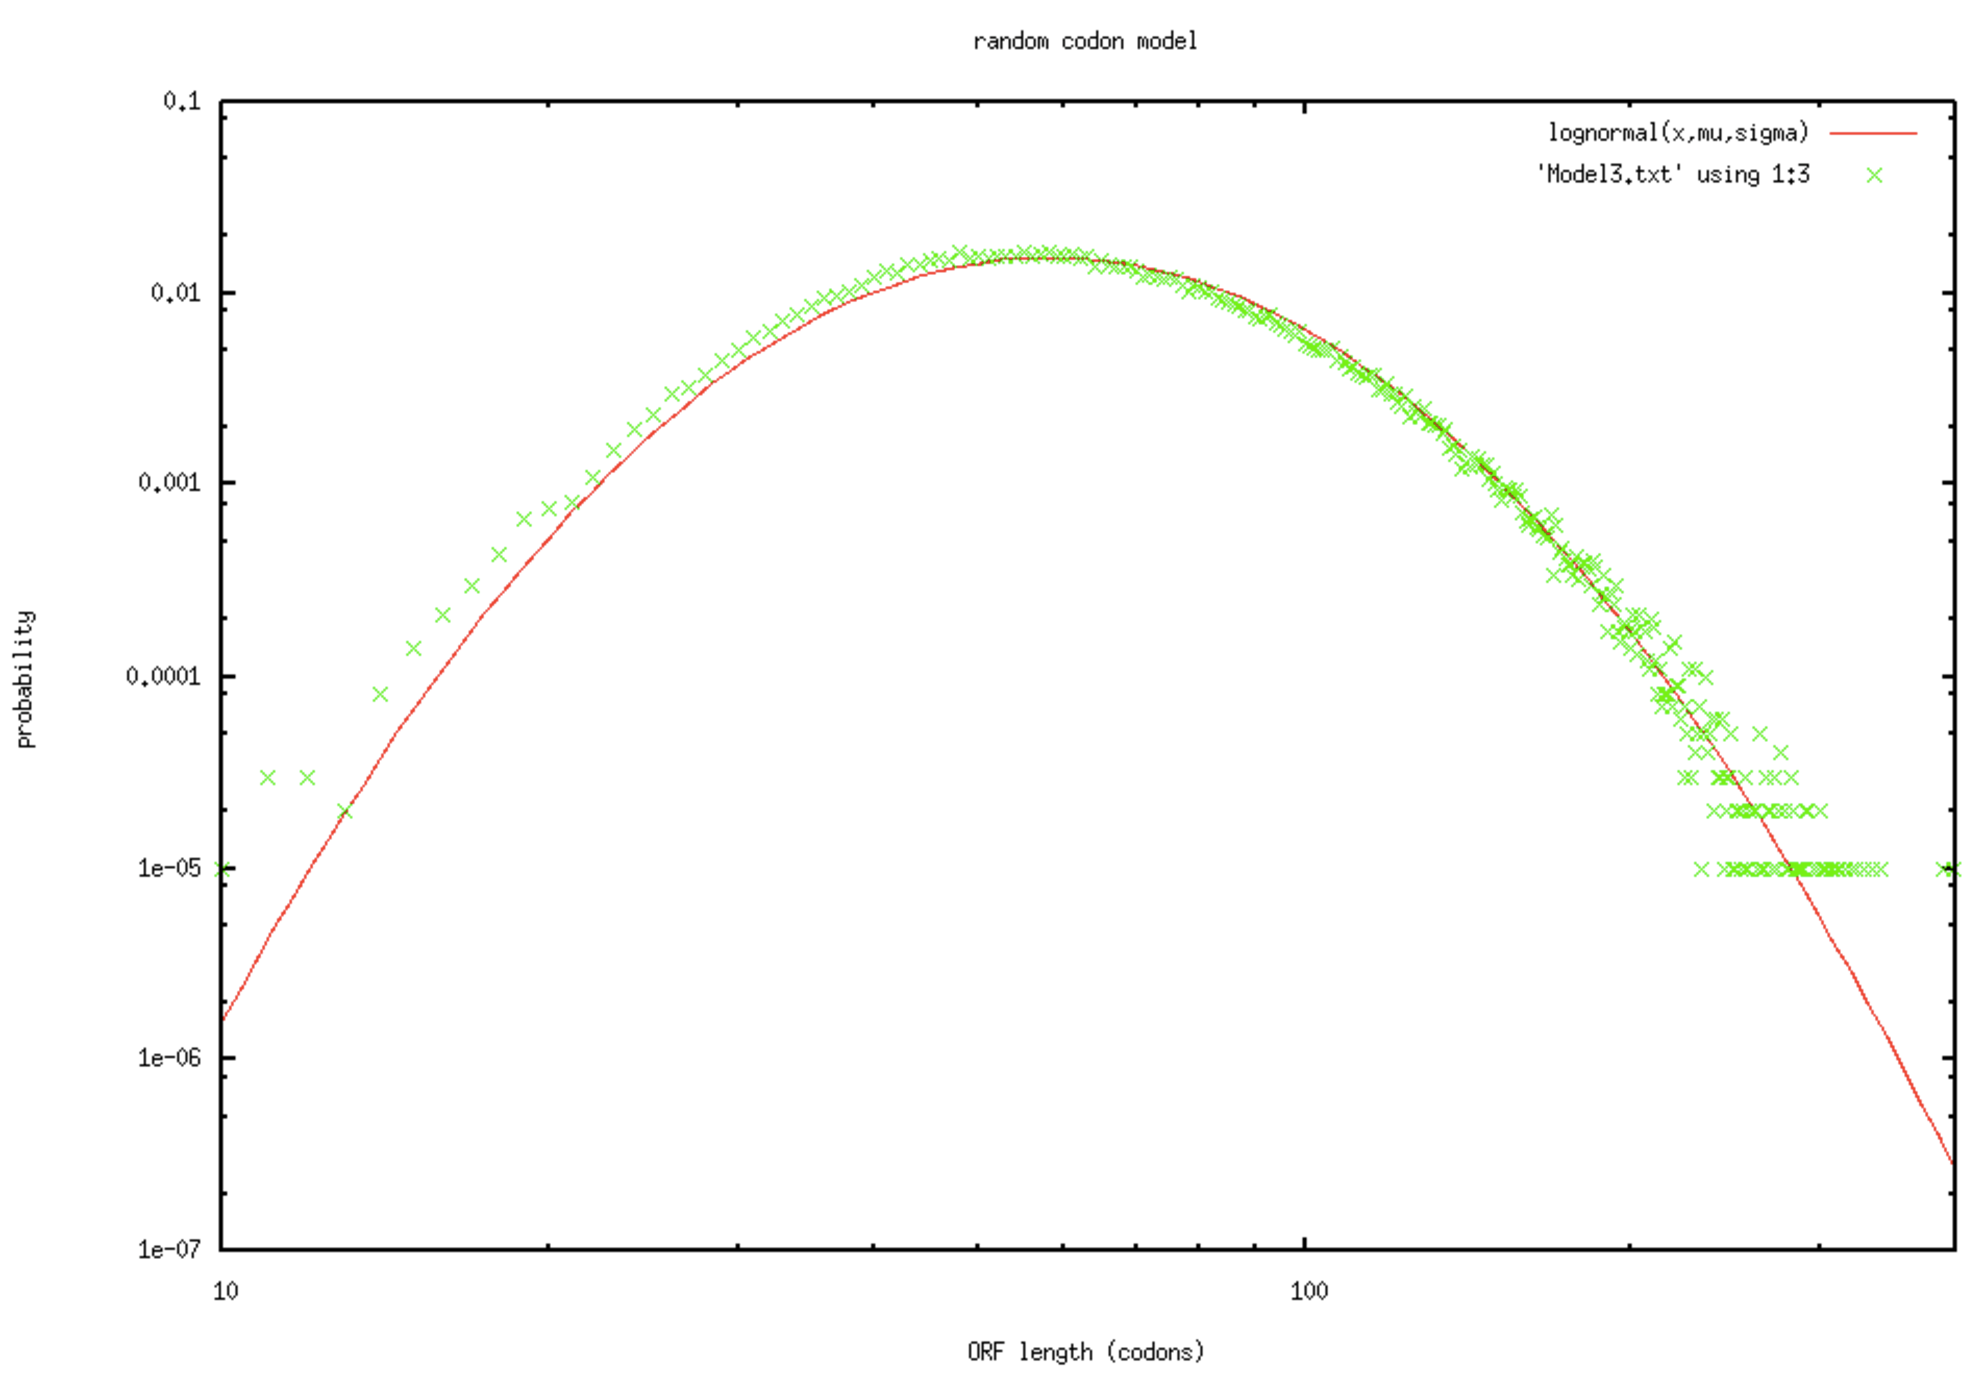
\includegraphics[width=\textwidth]{Model3LogProb.pdf} 
		\caption{Probability vs. ORF length}
        \end{subfigure}
        \begin{subfigure}[b]{0.49\textwidth}
                \centering
		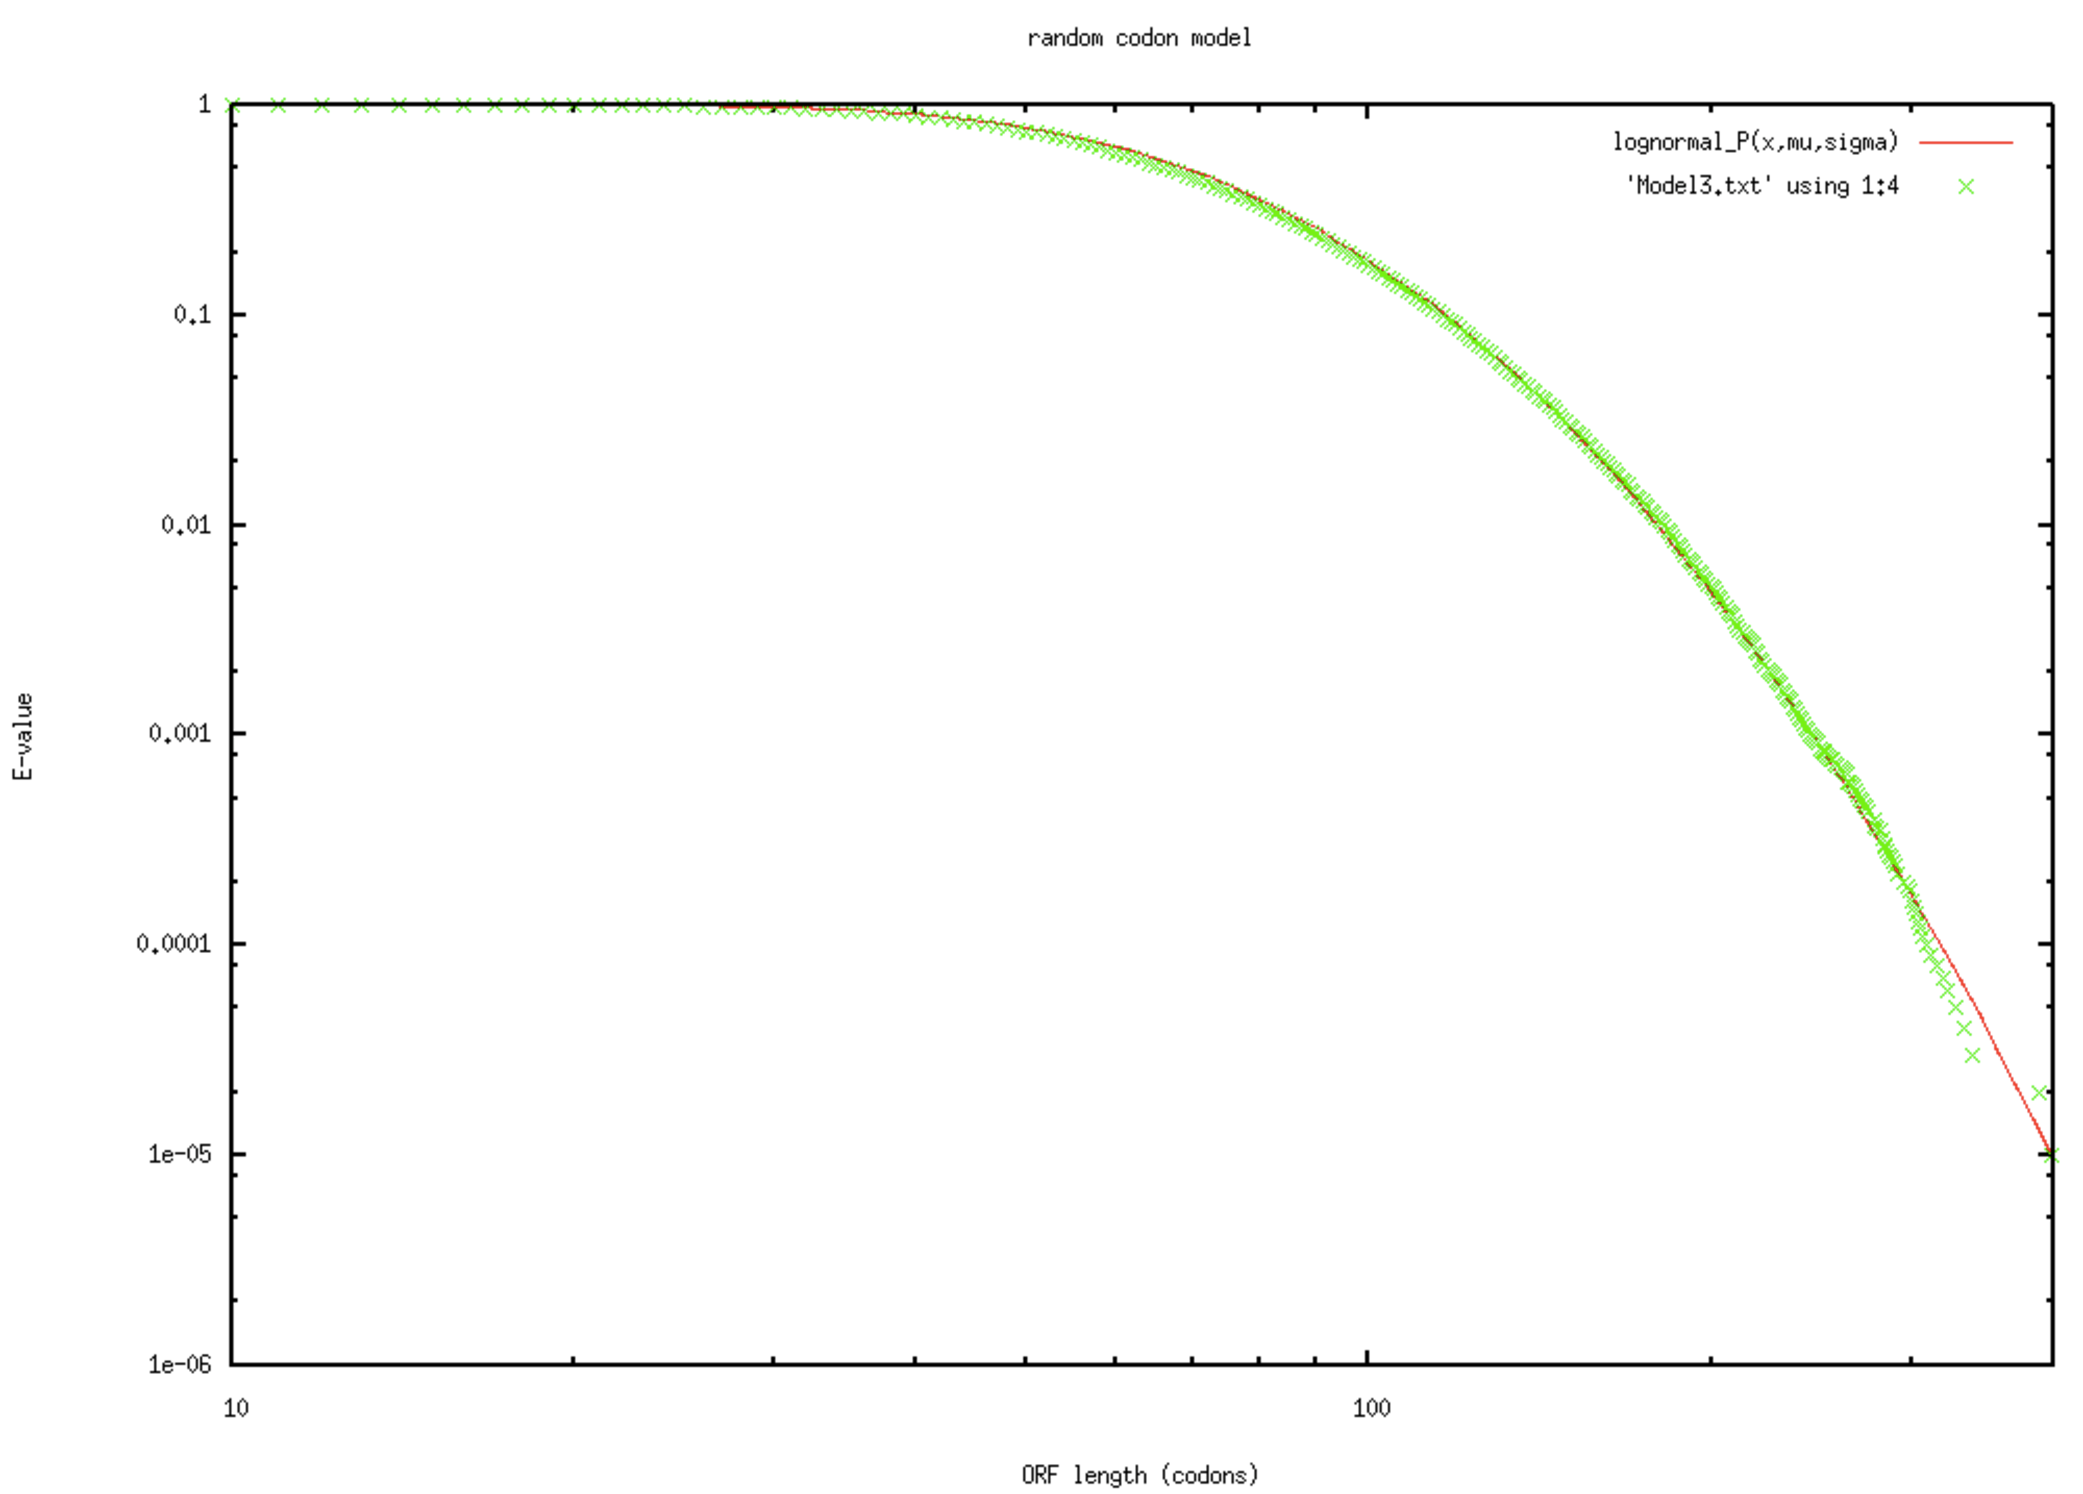
\includegraphics[width=\textwidth]{Model3LogE.pdf} 
		\caption{E-Value vs. ORF length}
        \end{subfigure}

        \caption{Lognormal Distribution for Random Codon Model}\label{fig:Model3Log}
\end{figure}

For the Gumbel distribution we get a p-value of $6.831454 \times 10^{-6}$.  Since there are 2994 genes in the species, we find the e-value to be 0.02047.  For the lognormal distribution we find a p-value of $1.32777 \times 10^{-5}$, which gives an e-value of 0.03975.  While both of these fall under the 5\% mark, it is harder to reject this null model.

\subsection{Null Model 4}
In this null model we randomly generate a series of codons that codes for THSA\_SULSH, using the codon biases of S. solfataricus.  After this ORF is generated, we take the reverse compliment and find the longest ORF.  We repeat this 100,000 times to get a distribution of ORF lengths.  Figure \ref{fig:Mode4Gum} shows our data fitted to a Gumbel distribution.  Figure \ref{fig:Model4Log} shows our data fitted to a lognormal distribution.

\begin{figure}[!htb]
        \centering
        \begin{subfigure}[b]{0.49\textwidth}
                \centering
		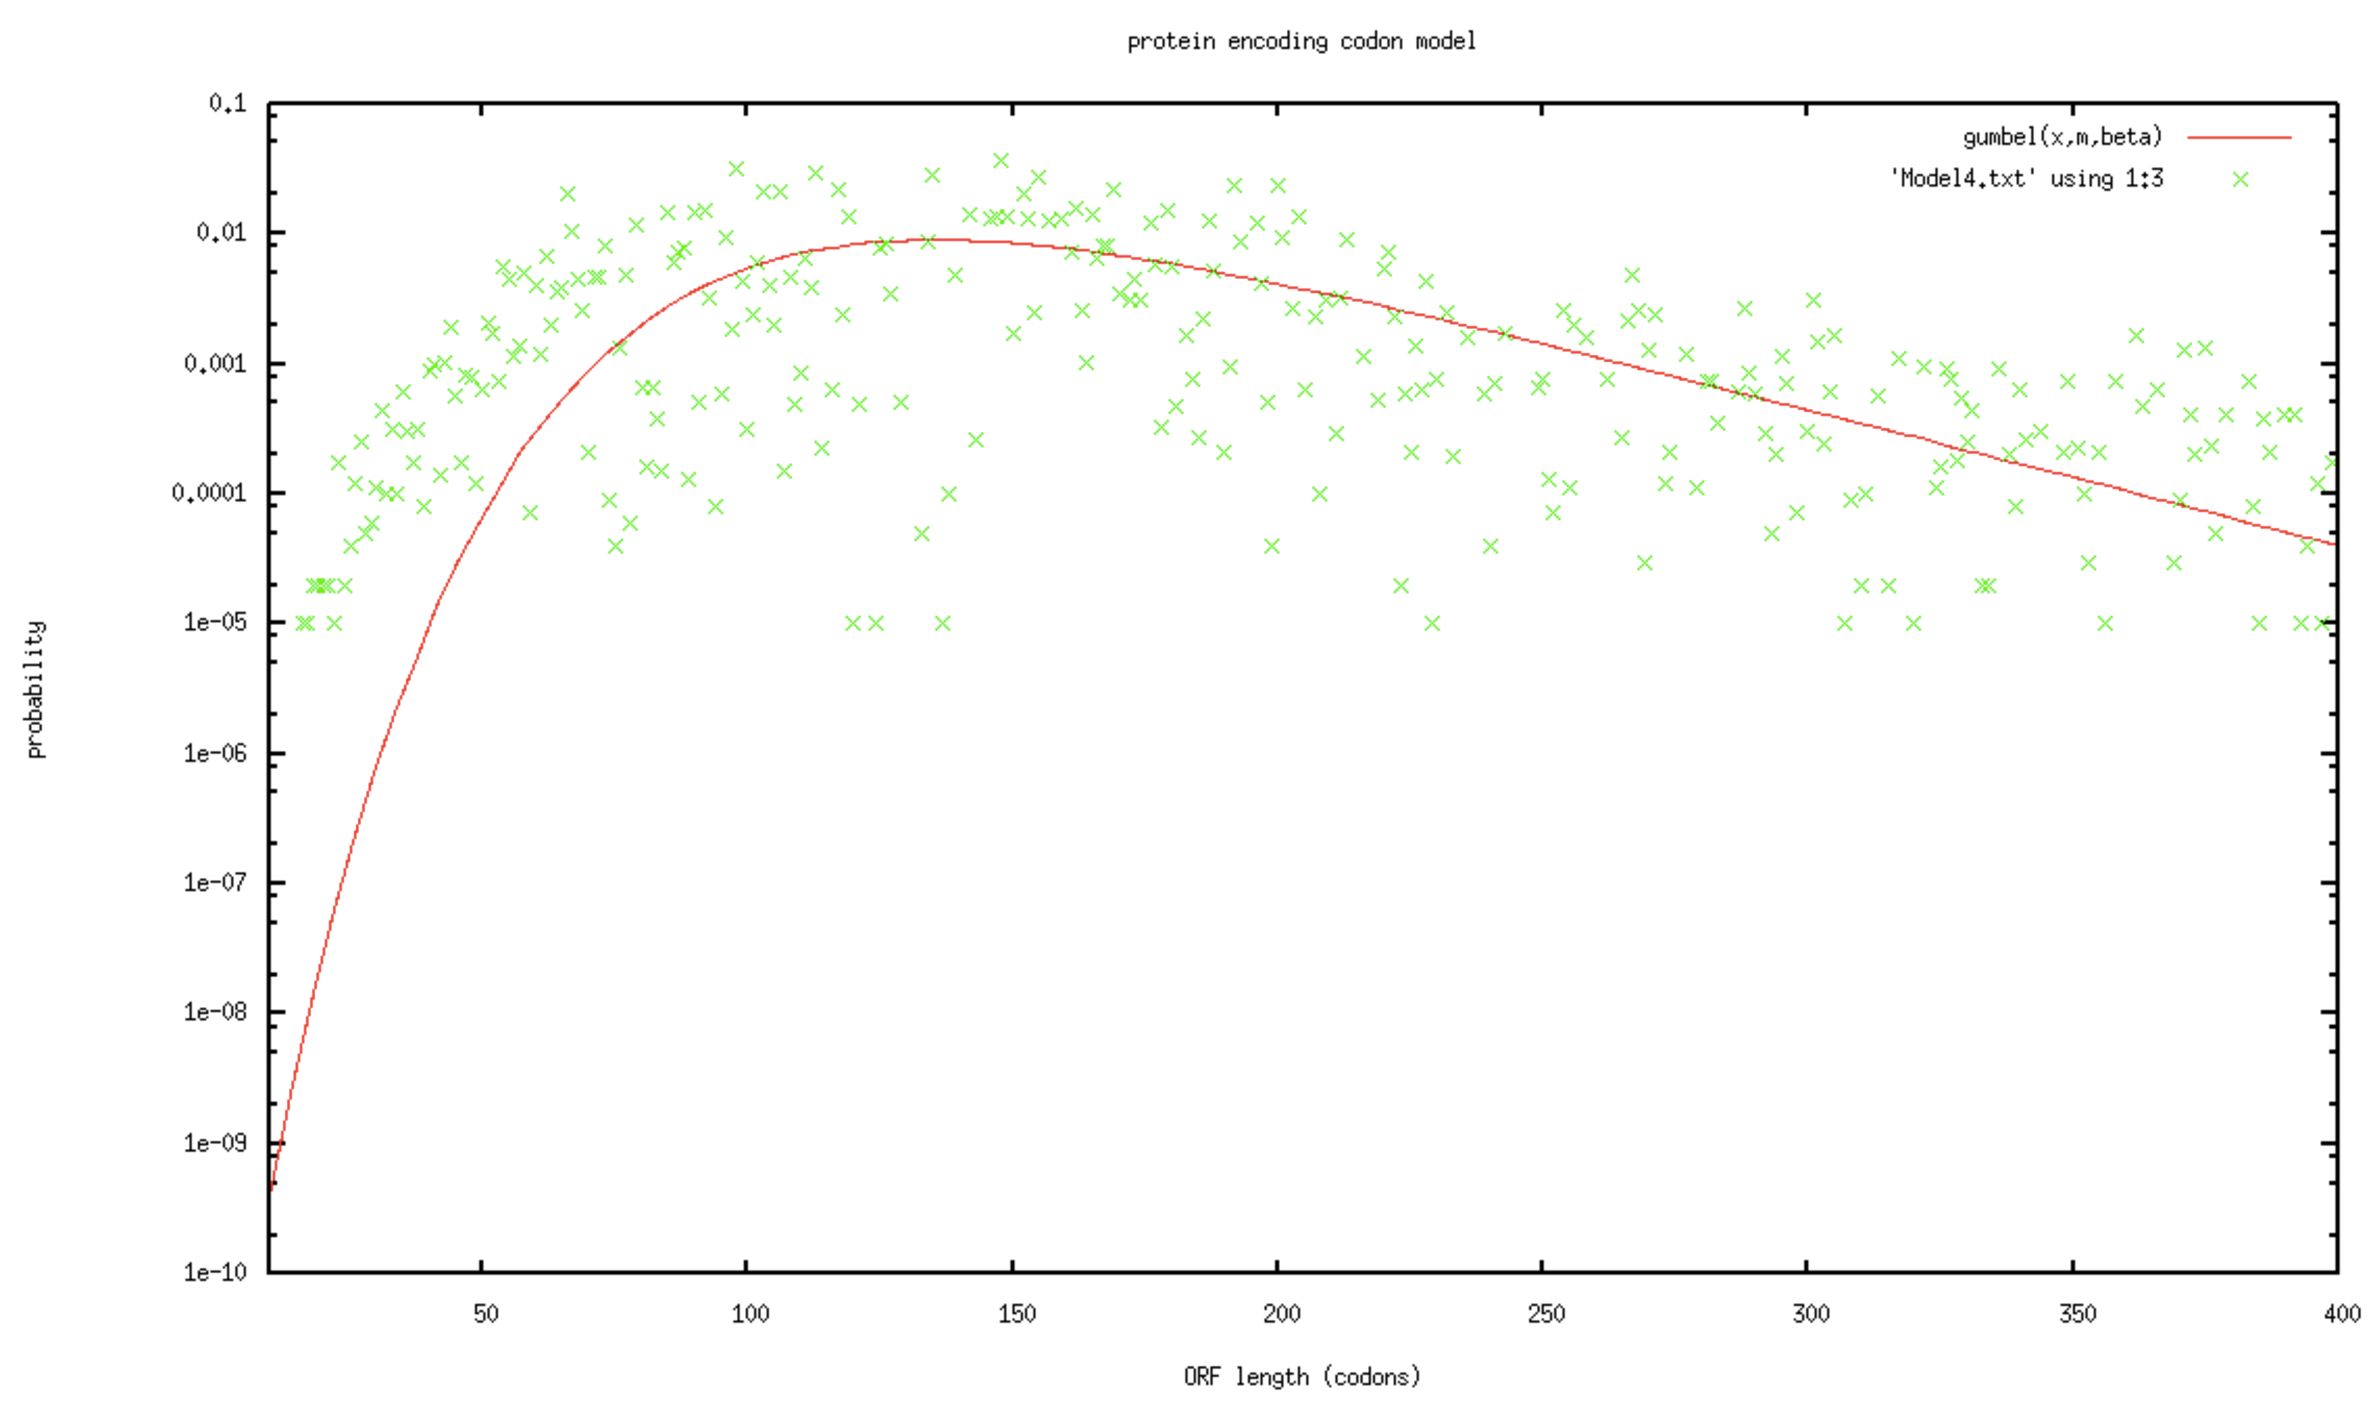
\includegraphics[width=\textwidth]{Model4GumProb.pdf} 
		\caption{Probability vs. ORF length}
        \end{subfigure}
        \begin{subfigure}[b]{0.49\textwidth}
                \centering
		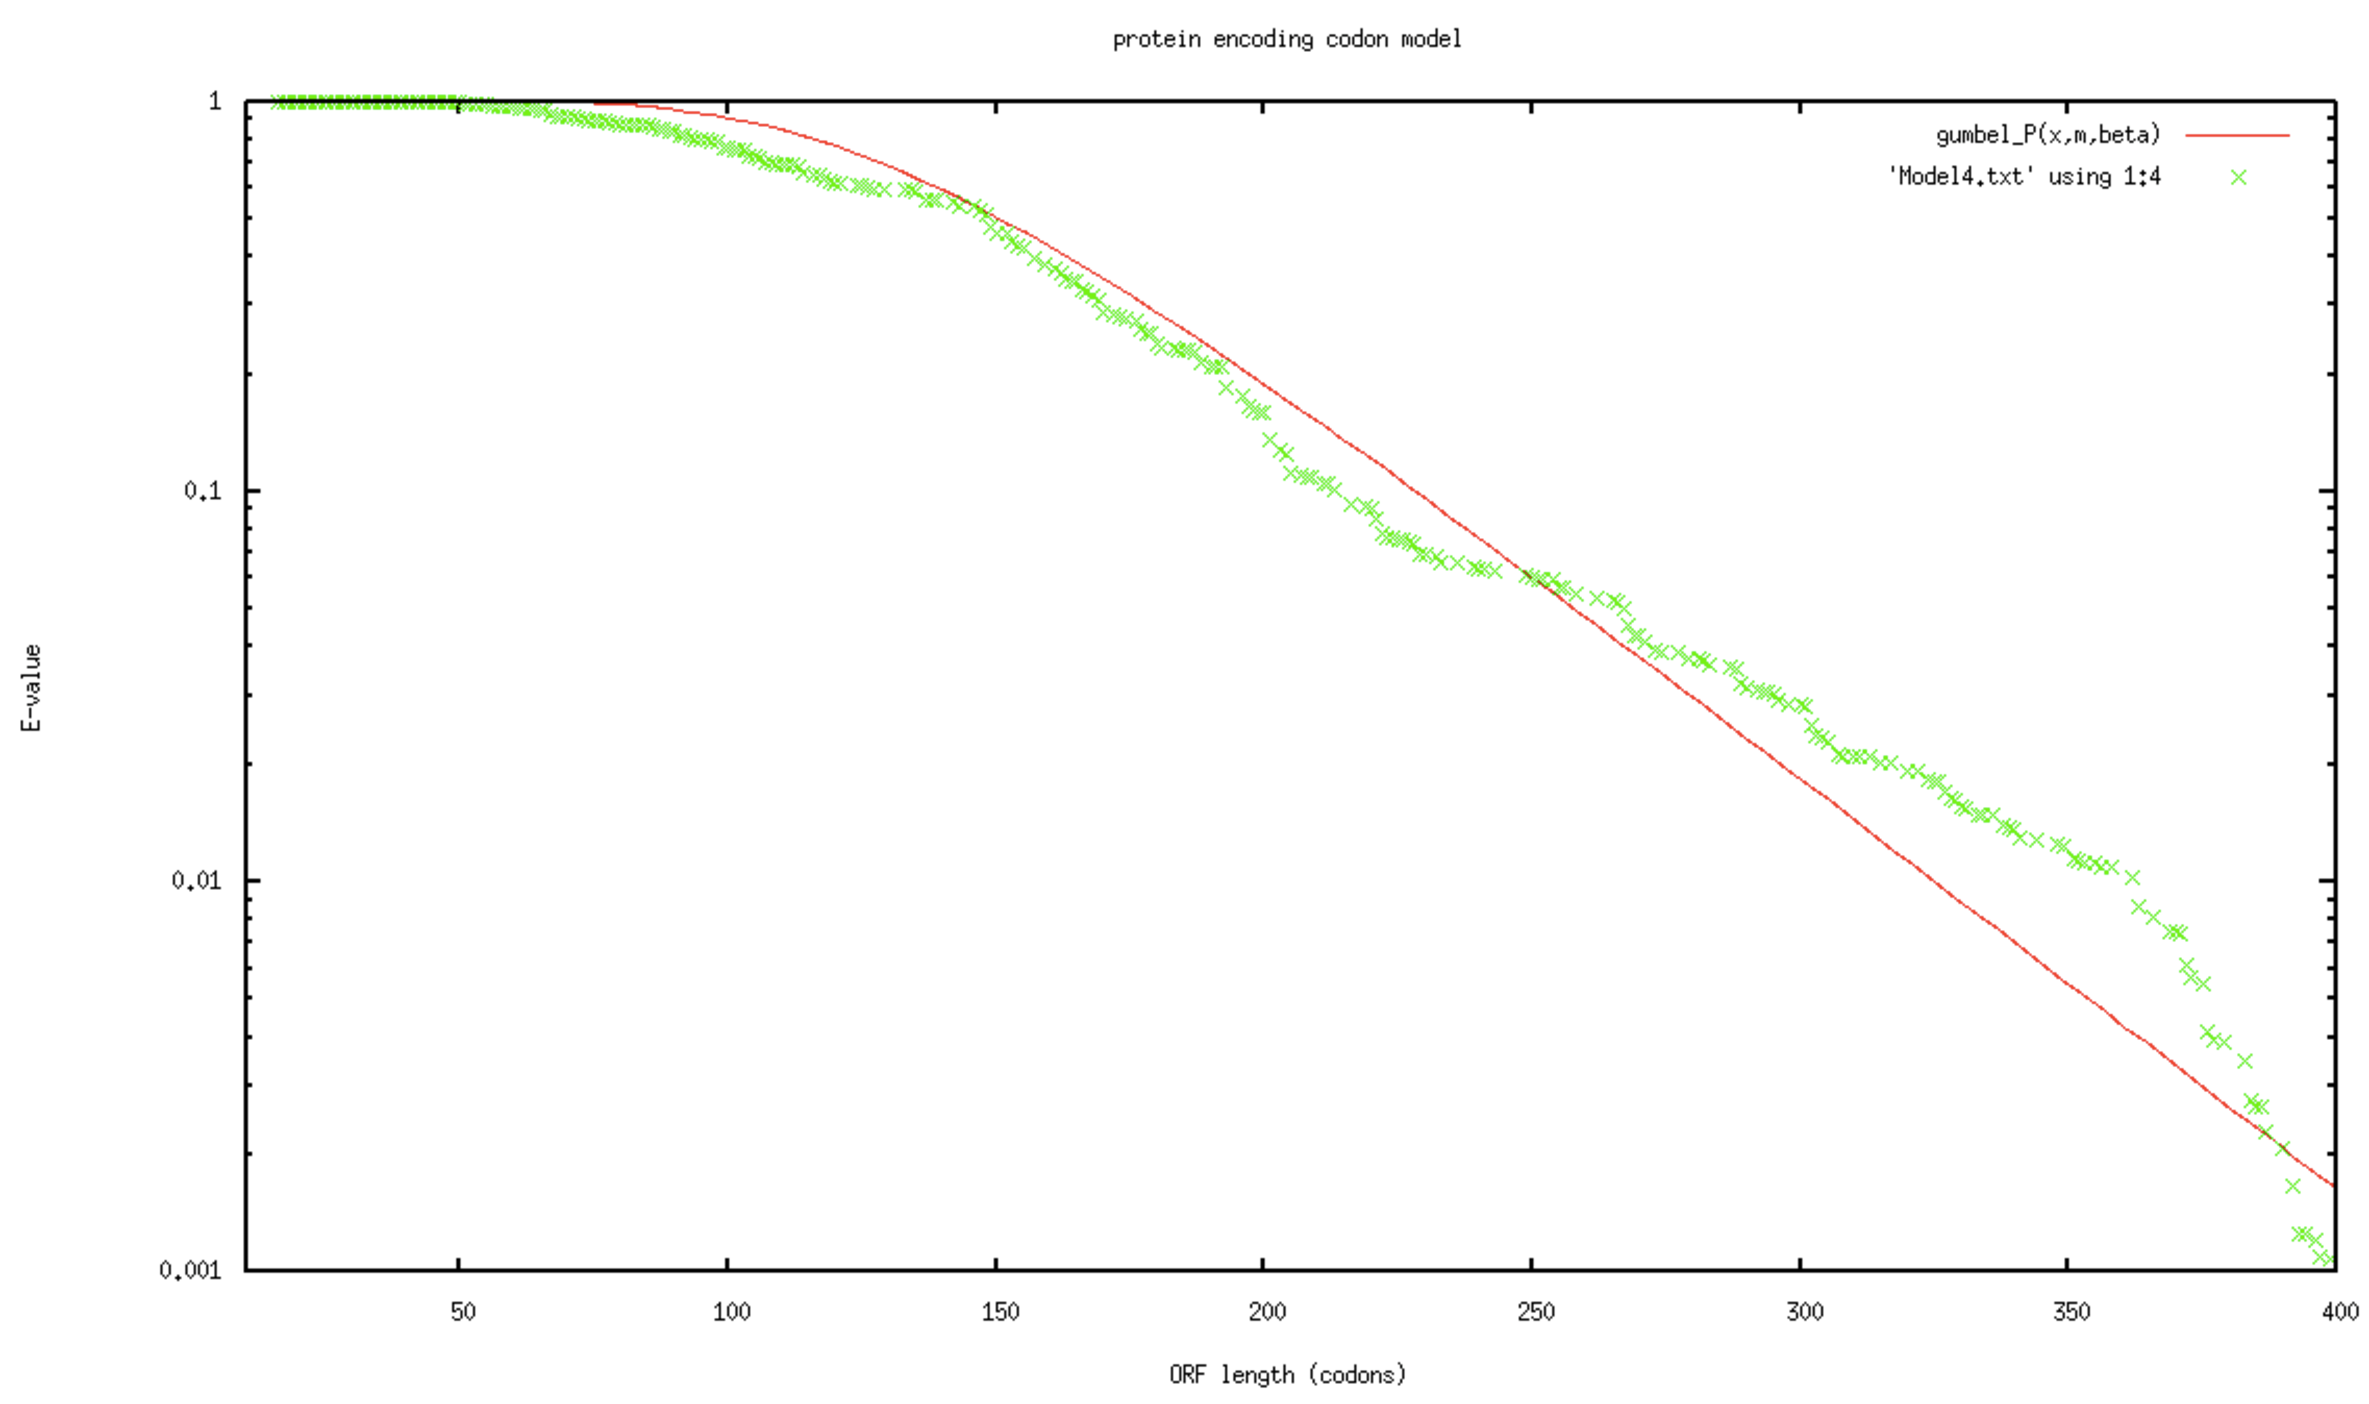
\includegraphics[width=\textwidth]{Model4GumE.pdf} 
		\caption{E-Value vs. ORF length}
        \end{subfigure}

        \caption{Gumbel Distribution for Protein Encoding Codon Model}\label{fig:Mode4Gum} 
\end{figure}

\begin{figure}[!htb]
        \centering
        \begin{subfigure}[b]{0.49\textwidth}
                \centering
		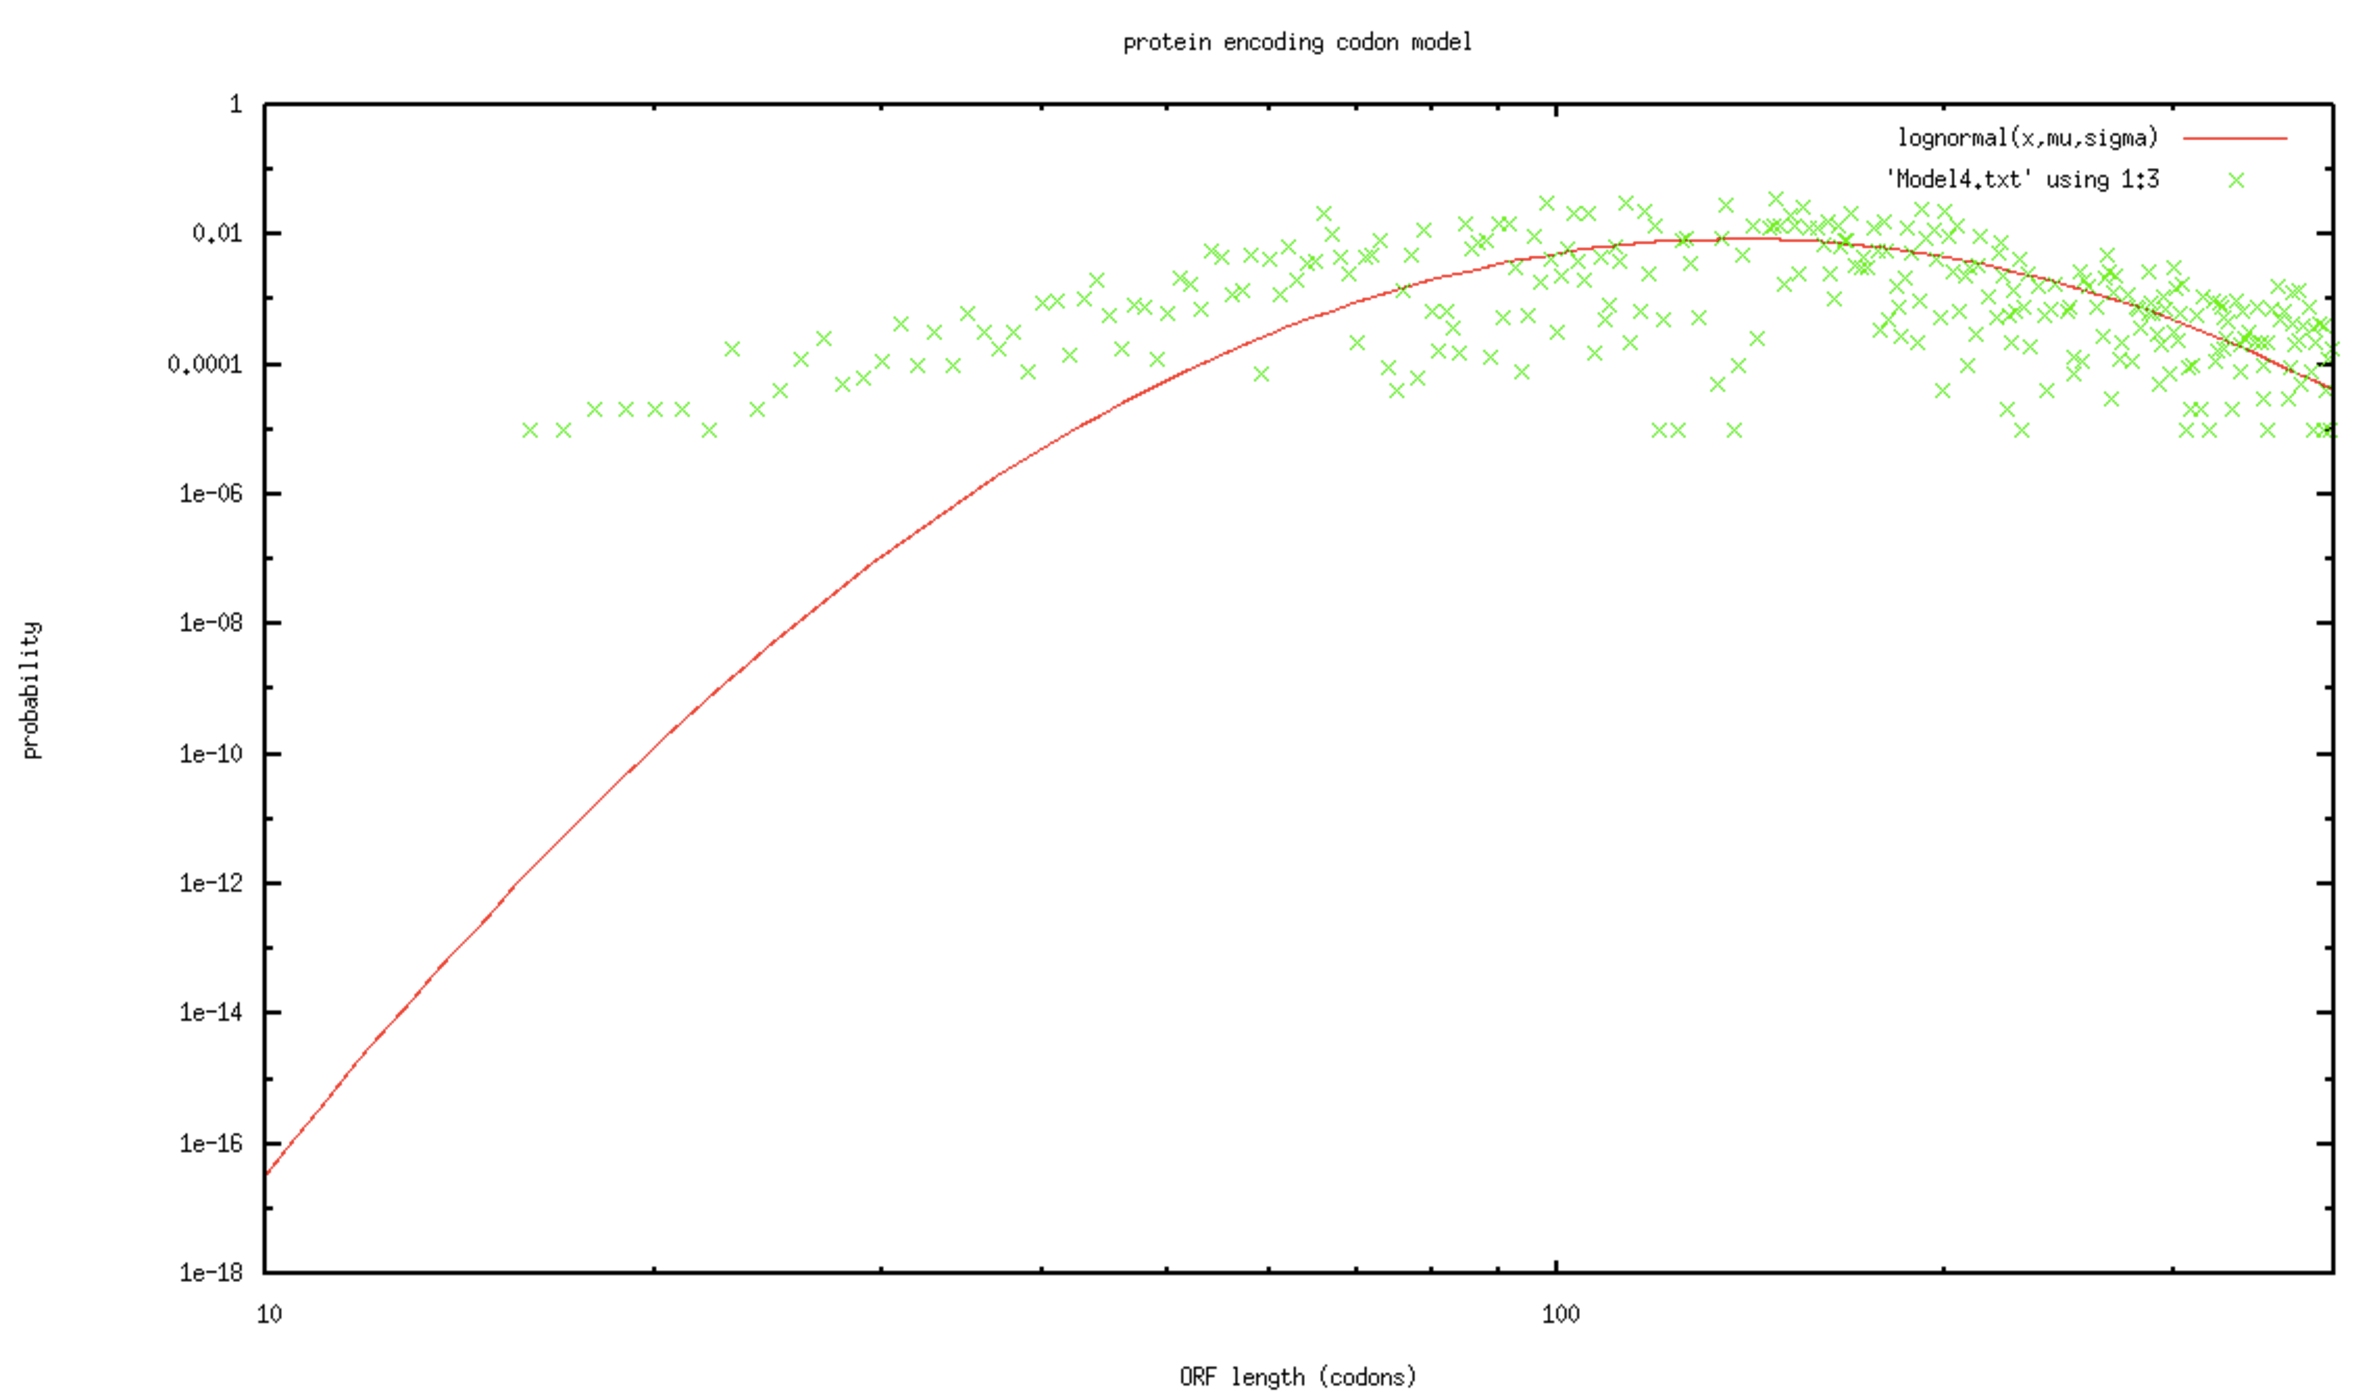
\includegraphics[width=\textwidth]{Model4LogProb.pdf} 
		\caption{Probability vs. ORF length}
        \end{subfigure}
        \begin{subfigure}[b]{0.49\textwidth}
                \centering
		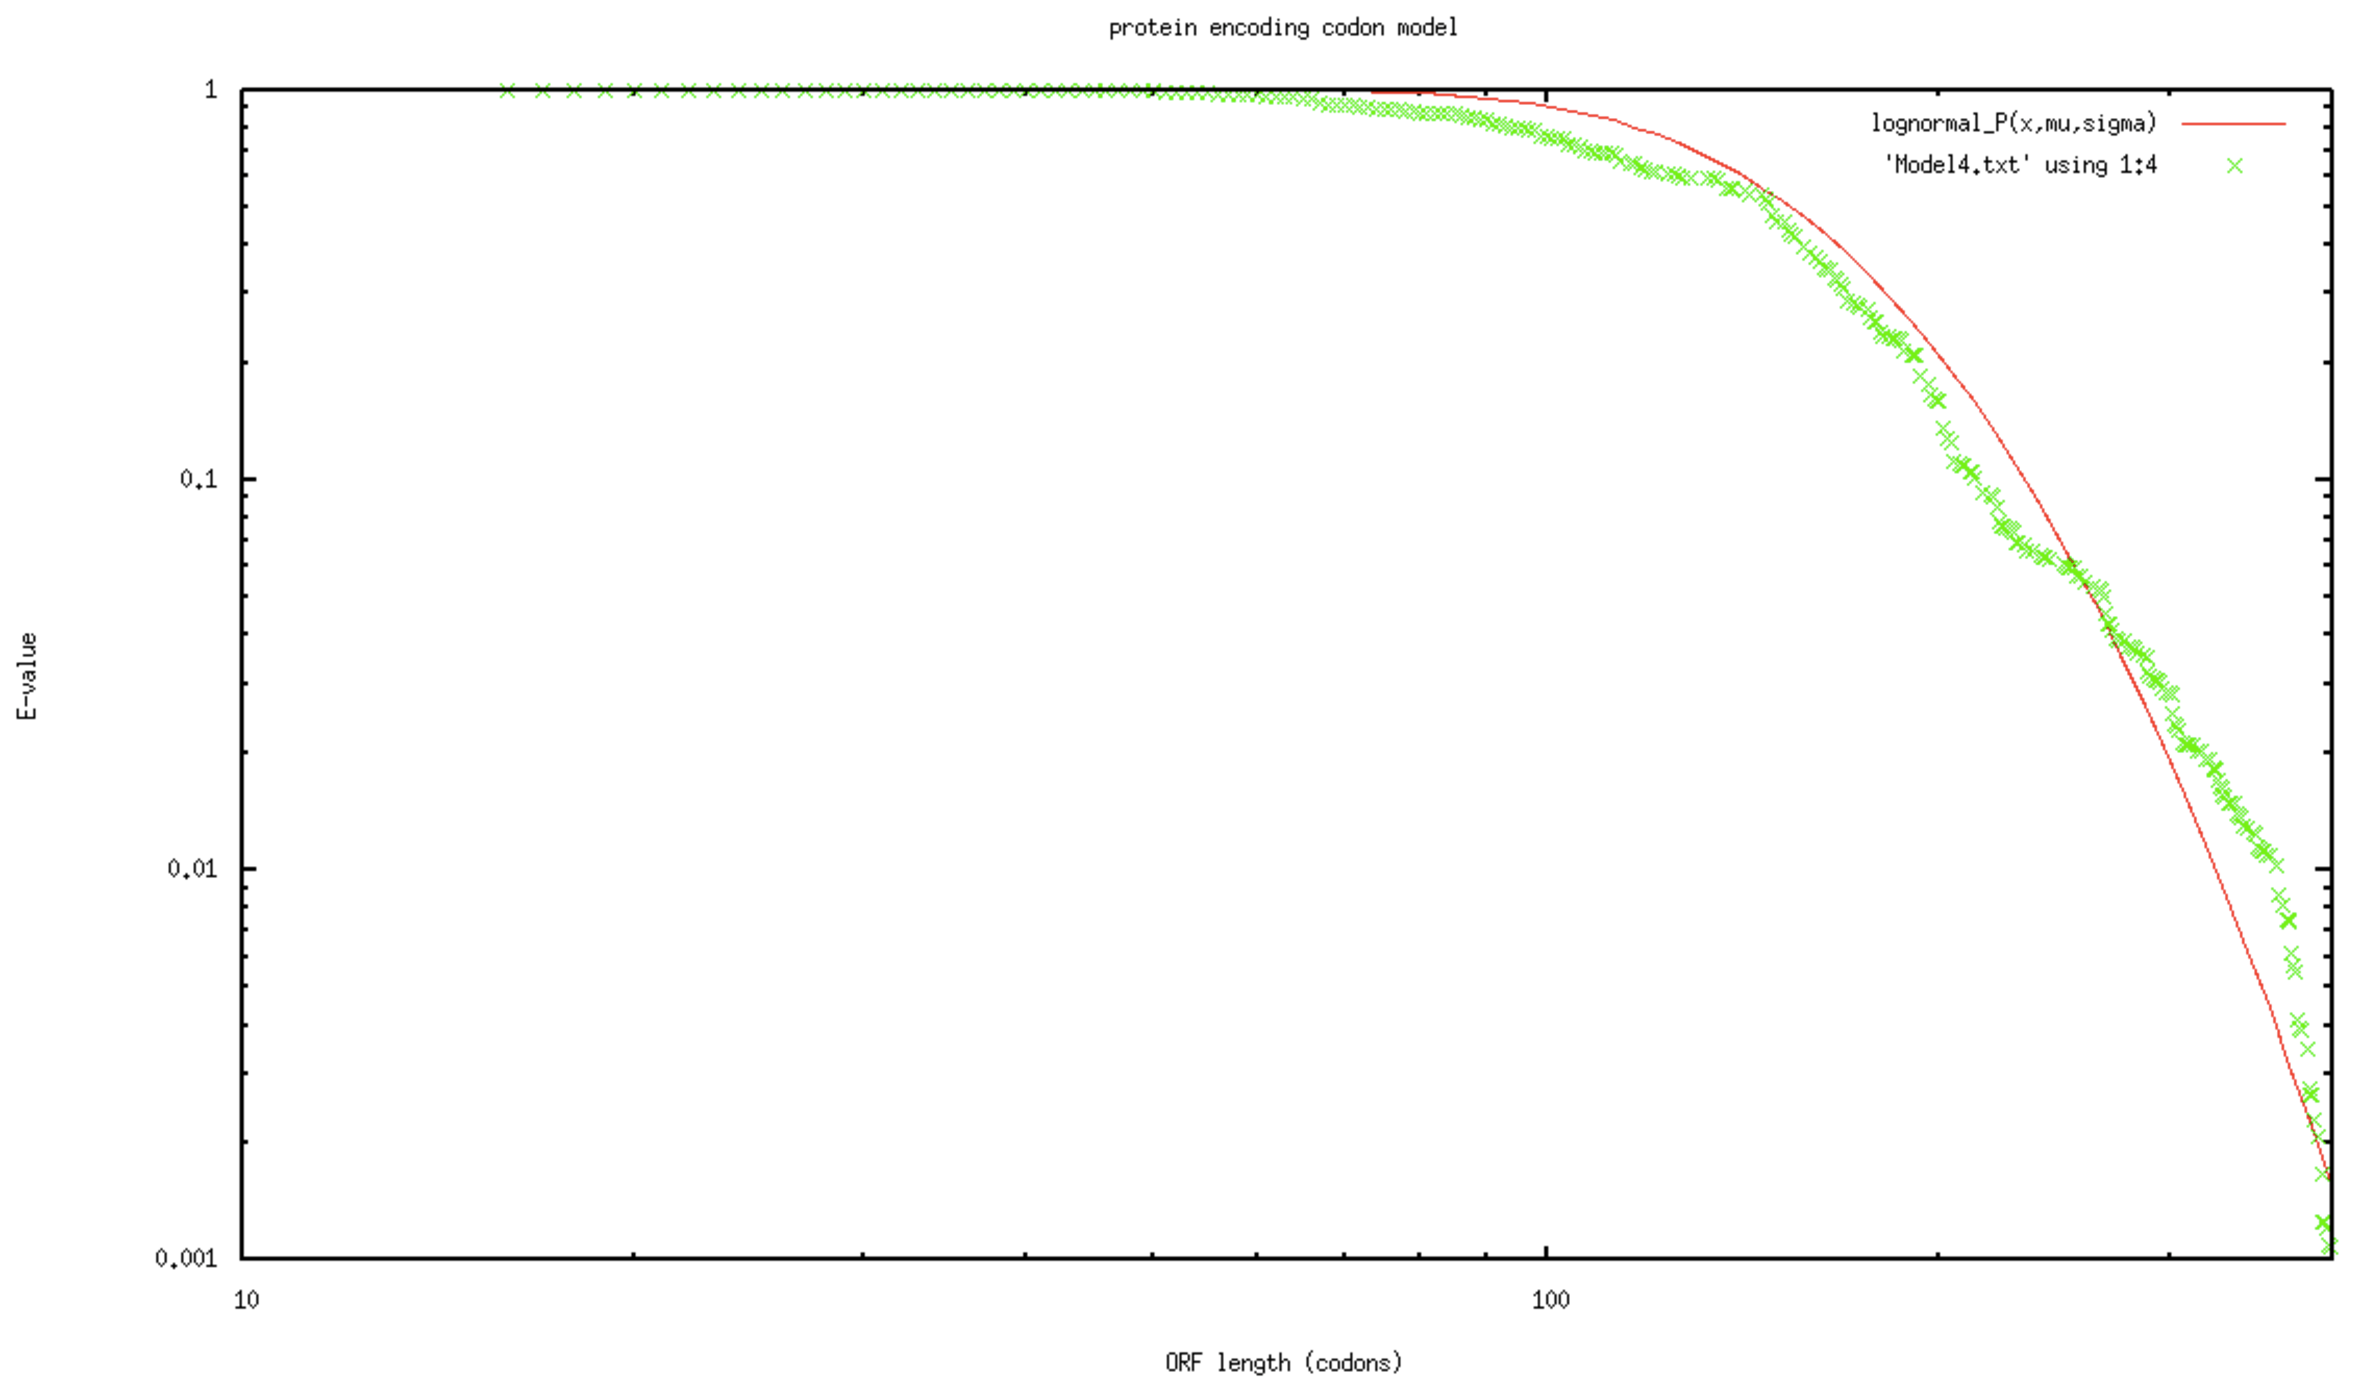
\includegraphics[width=\textwidth]{Model4LogE.pdf} 
		\caption{E-Value vs. ORF length}
        \end{subfigure}

        \caption{Lognormal Distribution for Protein Encoding Codon Model}\label{fig:Model4Log} 
\end{figure}

Since this data does not appear to fit either distribution that well, it does not make sense to use either in a cumulative function to find the p-value.  Instead we will estimate the p-value as the probability of getting an ORF of length 388 or longer from the counts in the histogram.  Here we find the p-value and e-value are both equal to 0.00207.  We can reject this null model at the 1\% confidence level, though not as confidently as we were able to reject null models 1 and 2.

\section{Conclusions}

The first two null models make it seem that finding an ORF of length 388 in S.solfataricus is very unlikely to happen by chance.  However the latter two null models are much less convincing.  It is hard to justify more laboratory work based purely on these results.

\end{document}